\subsection{Long-Slit Spectroscopy in L/M- and N-bands}

The purpose of the pipeline is to correct or remove contributions from
the instrument, telescope, and atmosphere and produce science-grade
data products for the L/M- and N-band \ac{LSS}
mode. Since the detector properties are not fully specified, especially of the new Geosnap, we currently assume
basically same reduction cascade for both spectral ranges LM and
N, respectively. The only major difference at the time being is the absence of \ac{WCU} laser sources in the N-band, which are only available during \ac{AIT} phase to generate a first guess of the pixel-to-wavelength relation. Therefore we assume a general first guess wavelength solution in the N-band based on that \ac{AIT} data. As we assume the instrument to be very stable, that approach should be sufficient for the low-resolution N-band spectroscopy. In the LM range, two fix-frequency lasers ($@3.39$µm and $@5.26$µm) and one tuneable ($4.68....4.78$µm) is foreseen in the \ac{WCU} to be taken on daily basis (cf. \cite{METIS-calibration_plan}). Although mainly foreseen to be used for the high-resolution spectroscopy \ac{LMS} mode, we can use these laser sources for the LM-band \ac{LSS} as well.

Special emphasis has to be drawn to the effects of the Earth's
atmosphere in several respects:
\begin{itemize}
\item Wavelength calibration: Absorption/emission features are intended to be
  used for the wavelength calibration. Thus, a good knowledge on /
  identification of these features is crucial for the accuracy of the
  wavelength calibration.
\item Telluric correction: In the MIR regime telluric absorption is
  one of the most dominant effects visible in spectra. Modelling
  approaches like \texttt{molecfit} heavily rely on accurate
  atmospheric input profiles, which represent the actual state and
  composition of the Earth's atmosphere. This especially applies to
  the \ac{PWV} content since this is the most
  dominant and most variable species.
\item Atmospheric dispersion: \ac{METIS} will have \ac{ADC}s compensating the
  effect of atmospheric dispersion. However, for technical reasons
  these ADCs are fixed at several positions. This means that the
  compensation is only partially. This leads to two practical effects:
  (a) wavelength-dependent slit losses, and (b) distortions in both,
  the spatial and the spectral direction (see \cite{METIS-ADC_study}
  for more details). For both, the pipeline needs to correct
  for. It is foreseen to determine these slitlosses on yearly basis with a separate calibration task (cf. \cite{METIS-calibration_plan}) and create a slit-loss table to be included in the static calibration database.
\end{itemize}

%However, to keep flexibility and independence of both branches, we
%define different recipes for the time being, although they will be
%mostly based on the same algorithms. We therefore focus here on the LM-band only.

Figure~\ref{Fig:LMLssAssomap} shows the reduction cascade and the association map for the recipes handling L/M-long-slit
spectroscopy data.  Table~\ref{Tab:LMLssDatProc} contains the data processing table for this mode. For the N-band \ac{LSS} mode the cascade and the data processing table is given in Fig.\ref{Fig:NLssAssomap} and Table~\ref{Tab:NLssDatProc}, respectively (cf. also Fig.~\ref{Fig:LSScascadelegend}).

In general, there are four major steps in each of the two cascades:
\begin{itemize}
    \item \textbf{Preparation step:} This contains the recipes, which are invoked only rarely, e.g. after major instrument interventions, or on monthly/yearly basis to update the static calibration database. In case of the \ac{LSS} pipeline this concerns the creation of the gain maps /linearity checks and the determination of the slit losses induced by the fixed positions of the ADCs (cf. Section "Calibration of slit losses" in Calibration plan \cite{METIS-calibration_plan}).
    \item \textbf{Basic steps}: The basic steps aim for correcting the detector influence, in particular the dark correction and the determination of the master \ac{RSRF}.
    \item \textbf{Calibration/correction steps}: This is the main part which incorporates the order trace detection, distortion, wavelength and flux correction.
    \item \textbf{Post-calibration steps}: After havig calibrated spectra at hand, the last step is the telluric absorption correction.
\end{itemize}

\begin{figure}[ht]
  \centering
  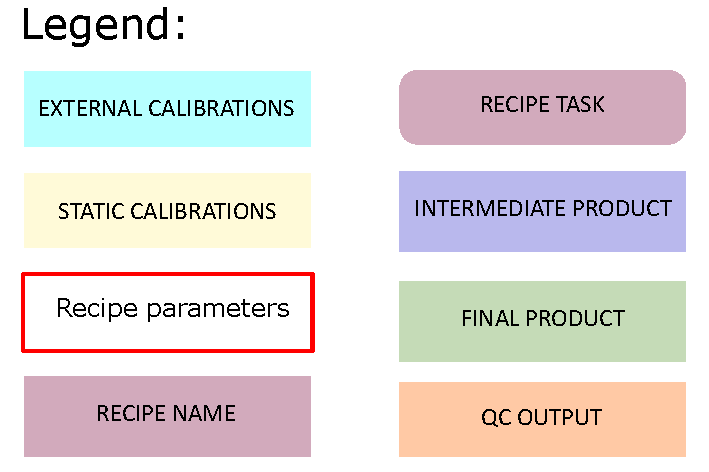
\includegraphics[width=0.4\textheight]{figures/legend.pdf}
  \caption[Legend]{Legend of the coloured boxes in the \ac{LSS} cascades.}
  \label{Fig:LSScascadelegend}
\end{figure}
\clearpage

\begin{sidewaysfigure}[ht]
  \centering
  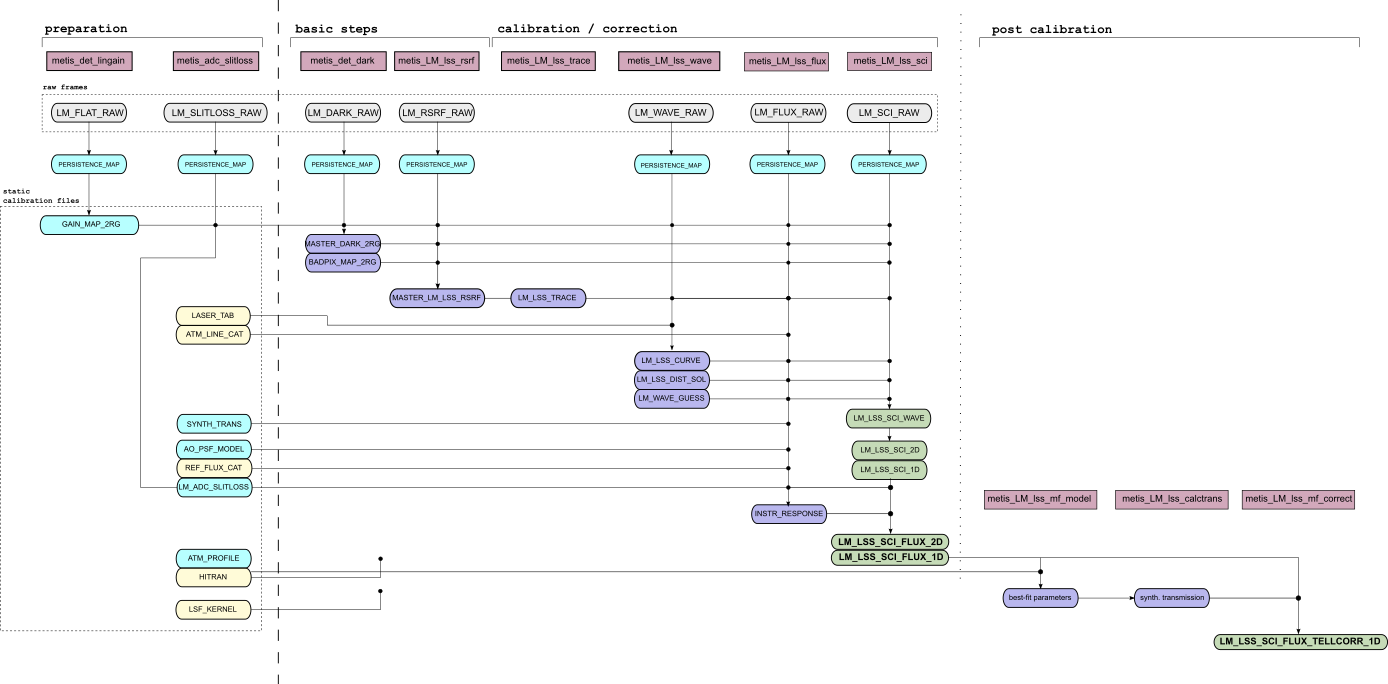
\includegraphics[width=0.9\textheight]{figures/LM_LSS_pipeline_wf_draft_latest_v0.72.png}
  \caption[Reduction cascade and association map for LM long-slit
  spectroscopy]{Reduction cascade and association map for long-slit
    spectroscopy in the LM bands.  }
  \label{Fig:LMLssAssomap}
\end{sidewaysfigure}



% \begin{sidewaysfigure}[ht]
%   \centering
%   \includegraphics[width=0.9\textheight]{figures/NQ_LSS_pipeline_wf_draft_latest.png}
%   \caption[Reduction cascade and association map for N long-slit
%   spectroscopy]{Reduction cascade and association map for long-slit
%     spectroscopy in the N band.  }
%   \label{Fig:NQLssAssomap}
% \end{sidewaysfigure}


%% ---- Table: LM long-slit spectroscopy
\begin{sidewaystable}
  \footnotesize
  \begin{center}
    \caption[Data Processing table for LM long-slit spectroscopy]{%
      Data Processing table for LM long-slit spectroscopy
      calibration mode}\bigskip
    \label{Tab:LMLssDatProc}
    \begin{tabular}{|l|l|l|l|l|l|}
      \hline
      Data Type   & Classification & Recipe (Level)	& FITS Keywords & CalibDB & Products\\
    (Templates) & Keywords	 & Processing steps	&		&	  &	\\
    \hline
    \TPL{DARK}	& \CODE{DPR.CATG==CALIB} & \REC{metis_det_dark} & Exposure time	&	& Averaged dark frame\\
    		& \CODE{DPR.TYPE==DARK}  &			&		&	& Bad pixel map\\
    		& \CODE{DPR.TECH==IMAGE}  &			&		&	& \\
    \hline
    \TPL{FLAT}	& \CODE{DPR.CATG==CALIB} & \REC{metis_LM_lss_rsrf}\hyperref{rec:lsslmrsrf} & Exposure time	& dark	& Averaged, normalized flatfield\\
    		& \CODE{DPR.TYPE==FLAT}  &			&		&	& Bad pixel map\\
    		& \CODE{DPR.TECH==SPECTRUM}  &			&		&	& \\
    \hline
         	& \CODE{DPR.CATG==CALIB} & \REC{metis_LM_lss_trace}\hyperref{rec:lsslmtrace} & Exposure time	& 	& Order location\\
    		& \CODE{DPR.TYPE==FLAT}  &			&		&	& (polynomial fit)\\
    		& \CODE{DPR.TECH==SPECTRUM}  &			&		&	& \\
    \hline
    \TPL{WAVE,LASER} & \CODE{DPR.CATG==CATG} & \REC{metis_LM_lss_wave}\hyperref{rec:lsslmwave} & Object name &  LASER\_TAB & wavelength solution\\
    		& \CODE{DPR.TYPE==WAVE,LASER}   &			   & Exposure time & &\\
    		& \CODE{DPR.TECH==SPECTRUM}  &			&		&	& \\
    		& \CODE{PRO.CATG==SPECTRUM}   &  &  & & \\
    \hline
    \TPL{FLUX,STD} & \CODE{DPR.CATG==CALIB} & \REC{metis_LM_lss_flux}\hyperref{rec:lsslmflux} & Object name (Flux STD) & reference flux of STD & Instrumental\\
    		& \CODE{DPR.TYPE==FLUX,STD}   &			   & Exposure time & ATM\_LINE\_CAT & response function\\
    		& \CODE{DPR.TECH==SPECTRUM}  &			&		&	SYNTH\_TRANS& \\
    		& \CODE{PRO.CATG==SPECTRUM}   &  &  & LM\_ADC\_SLITLOSSES & \\
    		& & & & REF\_FLUX\_CAT &\\
    		& & & & AO\_PSF\_MODEL &\\    \hline
    \TPL{SCIENCE} & \CODE{DPR.CATG==SCIENCE} & \REC{metis_LM_lss_sci}\hyperref{rec:lsslmsci} & Object name & ATM\_LINE\_CAT  & Science grade spectrum\\
    		& \CODE{DPR.TYPE==OBJECT}   &			   & Exposure time & LM\_ADC\_SLITLOSSES &\\
    		& \CODE{DPR.TECH==SPECTRUM}  &			&		&	& \\
    		& \CODE{PRO.CATG==SPECTRUM}   &  &  & & \\
    \hline
            & \CODE{DPR.CATG==SCIENCE} & \REC{metis_LM_lss_model} & Object name & \ac{LSF} Kernel	 & Best-fit \\
    		& \CODE{DPR.TYPE==OBJECT}   &			  & & atm. profile  & \texttt{molecfit} parameters\\
    		& \CODE{DPR.TECH==TBD}  &			&		& Line database	& \\
    		& \CODE{PRO.CATG==TBD}   &  &  & & \\
    \hline
            & \CODE{DPR.CATG==SCIENCE} & \REC{metis_LM_lss_calctrans} & Object name & best-fit parameters	 & synthetic \\
    		& \CODE{DPR.TYPE==LSS}   &		&	   & atm. profile  & Transmission curve\\
    		& \CODE{DPR.TECH==TBD}  &			&		& Line database	& \\
    		& \CODE{PRO.CATG==TBD}   &  &  & & \\
    \hline
            & \CODE{DPR.CATG==SCIENCE} & \REC{metis_LM_lss_correct} & Object name & 	 & Absorption corrected\\
    		& \CODE{DPR.TYPE==LSS}   &			   & synthetic Transmission curve & & science spectrum\\
    		& \CODE{DPR.TECH==TBD}  &			&		&	& \\
    		& \CODE{PRO.CATG==TBD}   &  &  & & \\
    \hline
    \end{tabular}
  \end{center}
\end{sidewaystable}

\begin{sidewaysfigure}[ht]
  \centering
  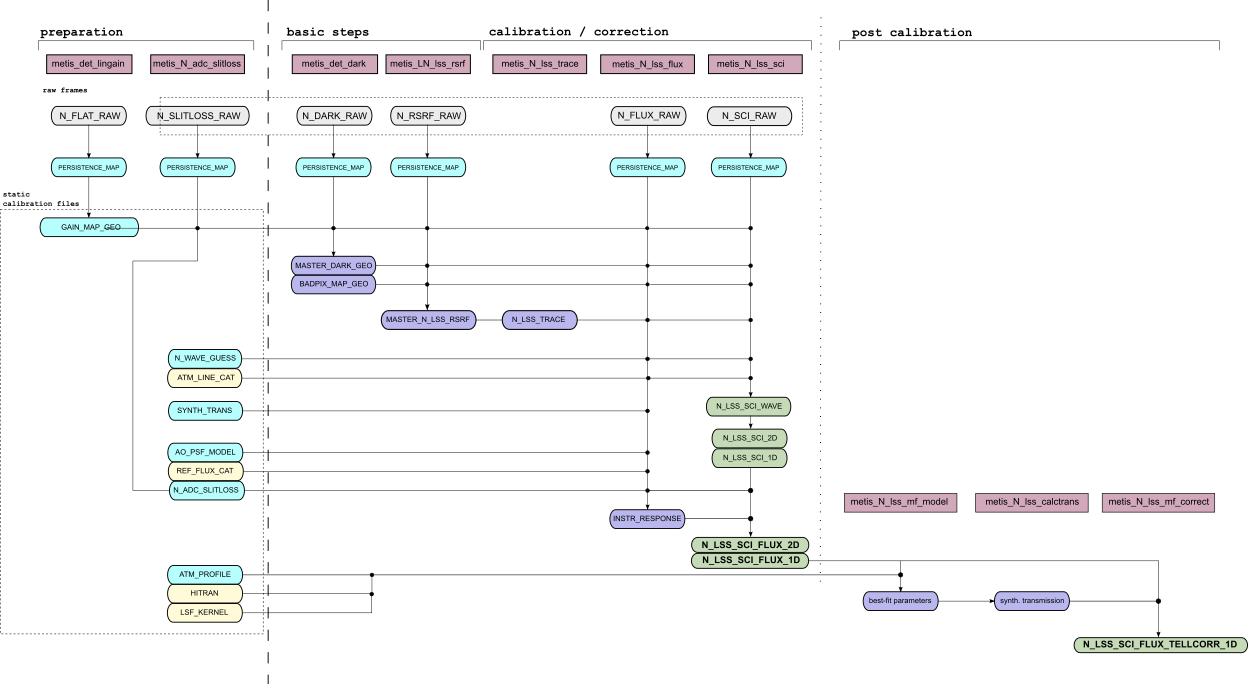
\includegraphics[width=0.9\textheight]{figures/N_LSS_pipeline_wf_draft_latest_v0.72.png}
  \caption[Reduction cascade and association map for N long-slit
  spectroscopy]{Reduction cascade and association map for long-slit
    spectroscopy in the N bands.  }
  \label{Fig:NLssAssomap}
\end{sidewaysfigure}

%% ---- Table: N long-slit spectroscopy
\begin{sidewaystable}
  \footnotesize
  \begin{center}
    \caption[Data Processing table for N-band long-slit spectroscopy]{%
      Data Processing table for N long-slit spectroscopy
      calibration mode}\bigskip
    \label{Tab:NLssDatProc}
    \begin{tabular}{|l|l|l|l|l|l|}
      \hline
      Data Type   & Classification & Recipe (Level)	& FITS Keywords & CalibDB & Products\\
    (Templates) & Keywords	 & Processing steps	&		&	  &	\\
    \hline
    \TPL{DARK}	& \CODE{DPR.CATG==CALIB} & \REC{metis_det_dark} & Exposure time	&	& Averaged dark frame\\
    		& \CODE{DPR.TYPE==DARK}  &			&		&	& Bad pixel map\\
    		& \CODE{DPR.TECH==IMAGE}  &			&		&	& \\
    \hline
    \TPL{FLAT}	& \CODE{DPR.CATG==CALIB} & \REC{metis_N_lss_rsrf}\hyperref{rec:lsslmrsrf} & Exposure time	& dark	& Averaged, normalized flatfield (\ac{RSRF}\\
    		& \CODE{DPR.TYPE==FLAT}  &			&		&	& Bad pixel map\\
    		& \CODE{DPR.TECH==SPECTRUM}  &			&		&	& \\
    \hline
         	& \CODE{DPR.CATG==CALIB} & \REC{metis_N_lss_trace}\hyperref{rec:lsslmtrace} & Exposure time	& 	& Order location\\
    		& \CODE{DPR.TYPE==FLAT}  &			&		&	& (polynomial fit)\\
    		& \CODE{DPR.TECH==SPECTRUM}  &			&		&	& \\
    \hline
    \TPL{FLUX,STD} & \CODE{DPR.CATG==CALIB} & \REC{metis_N_lss_flux}\hyperref{rec:lssnflux} & Object name (Flux STD) & reference flux of STD & Instrumental\\
    		& \CODE{DPR.TYPE==FLUX,STD}   &			   & Exposure time & N\_WAVE\_GUESS & response function\\
    		& \CODE{DPR.TECH==SPECTRUM}   &			   &		& ATM\_LINE\_CAT	& \\
    		& \CODE{PRO.CATG==SPECTRUM}   &  &  & SYNTH\_TRANS & \\
    		& & & & N\_ADC\_SLITLOSSES &\\
    		& & & & REF\_FLUX\_CAT &\\
    		& & & & AO\_PSF\_MODEL &\\
    \hline
    \TPL{SCIENCE} & \CODE{DPR.CATG==SCIENCE} & \REC{metis_N_lss_sci}\hyperref{rec:lssnsci} & Object name & N\_WAVE\_GUESS  & Science grade spectrum\\
    		& \CODE{DPR.TYPE==OBJECT}   &			   & Exposure time &  ATM\_LINE\_CAT &\\
    		& \CODE{DPR.TECH==SPECTRUM}  &			&		& N\_ADC\_SLITLOSSES	& \\
    		& \CODE{PRO.CATG==SPECTRUM}   &  &  &  & \\
    \hline
            & \CODE{DPR.CATG==SCIENCE} & \REC{metis_N_lss_model} & Object name & \ac{LSF} Kernel	 & Best-fit \\
    		& \CODE{DPR.TYPE==OBJECT}   &			  & & atm. profile  & \texttt{molecfit} parameters\\
    		& \CODE{DPR.TECH==TBD}  &			&		& Line database	& \\
    		& \CODE{PRO.CATG==TBD}   &  &  & & \\
    \hline
            & \CODE{DPR.CATG==SCIENCE} & \REC{metis_N_lss_calctrans} & Object name & best-fit parameters	 & synthetic \\
    		& \CODE{DPR.TYPE==LSS}   &		&	   & atm. profile  & Transmission curve\\
    		& \CODE{DPR.TECH==TBD}  &			&		& Line database	& \\
    		& \CODE{PRO.CATG==TBD}   &  &  & & \\
    \hline
            & \CODE{DPR.CATG==SCIENCE} & \REC{metis_N_lss_correct} & Object name & 	 & Absorption corrected\\
    		& \CODE{DPR.TYPE==LSS}   &			   & synthetic Transmission curve & & science spectrum\\
    		& \CODE{DPR.TECH==TBD}  &			&		&	& \\
    		& \CODE{PRO.CATG==TBD}   &  &  & & \\
    \hline
    \end{tabular}
  \end{center}
\end{sidewaystable}